
\subsection{SMR的dataflow}
这一节将介绍新的mapreduce系统\myds 的运行时,
相比已有的工作,\myds 所做的改进工作
\subsection{流水线并行}
%主要讲述流水线并行的优势,以及各个部件,上层能够看到的,下一章再来详细介绍底层实现上的支持
如上问所述,影响Phoenix性能的关键因素是
barrier的存在,
以及Posix线程库较差的scalability。
DMR基于一种新的Producer-Consumer模型,
打破barrier,且不再使用线程库,
从而提高处理的效率和scalability。
本节阐述新的Producer-Consumer的设计原理,
DMR的流水并行,以及地址空间的隔离。


\subsubsection{produce-consume模型}
%将详细介绍这个producer-consumer模型的所有特点,
如上所述,map worker和reducer worker的流水执行,
需要底层Producer-Consumer模型的支持,
本节将详细描述该模型的设计原理。

通常producer-consumer模型中,
producer和consumer之间有一个queue,
producer向queue中添加任务,
consumer从queue中读取任务。
MRPhi\cite{lu2013mrphi}为了使Map和Reduce并行执行,
便是采用这种Producer-Consumer模型,
具体如图\ref{mrphi:pc-model}所示。
在这个模型中,每个reduce worker对应一个queue,
map worker产生的数据会追加到queue中,
这是一个多对一的produce-consume模型,
\begin{figure}[!h!t]  
    \centering
    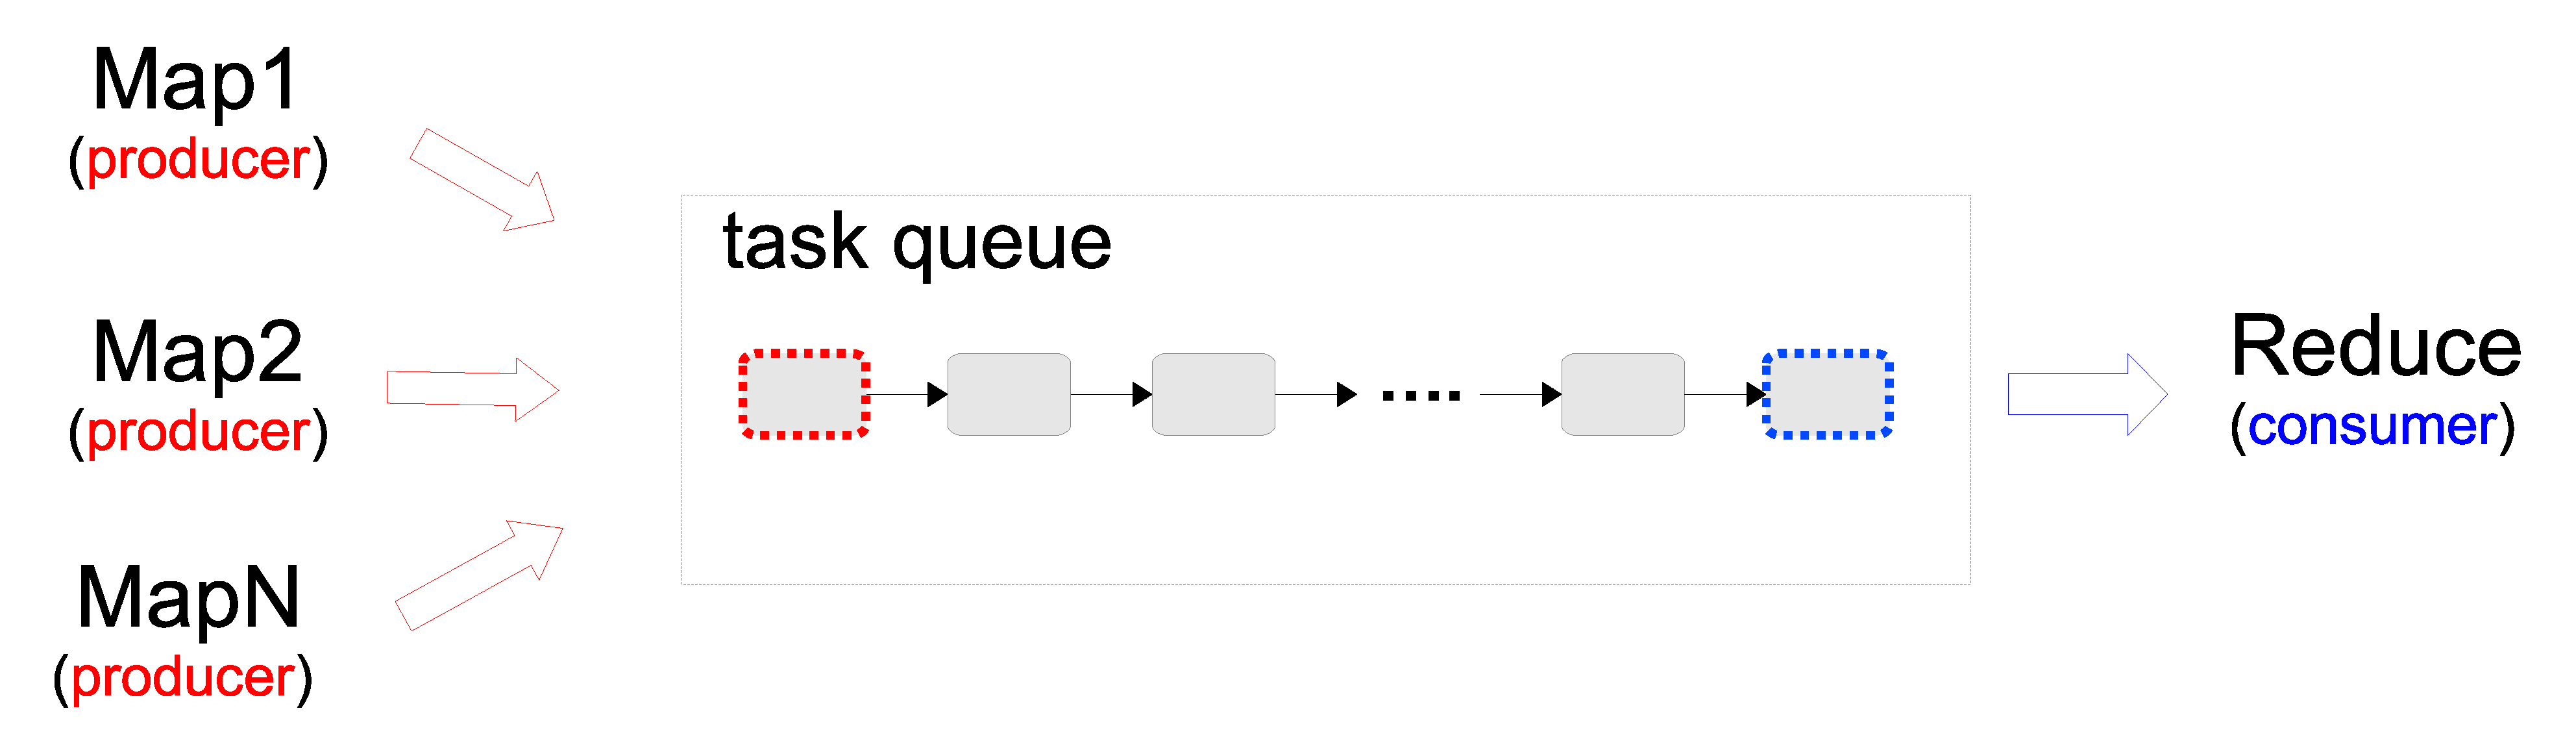
\includegraphics[width=0.5\textwidth]{img/mrphi_pc_model.eps}
    \caption{producer-consumer model in MRPhi}
    \label{mrphi:pc-model}
\end{figure}
虽然MRPhi利用该produce-consume模型实现的Map和Reduce阶段的并发执行,
但是它存在以下两个问题:
\begin{itemize}  
  \item map worker将task插入到queue中之前,需要竞争queue的lock。
  并且线程数越多时,等待lock的开销会越大。
  由于多个map worker同时向task queue中插入任务,
  需要一定的同步机制保证插入的正确性,
  这会造成一定的等待开销。
  \item queue的管理问题,虽然MRPhi\cite{lu2013mrphi}中并没有提到,
  具体的queue是如何管理的,但queue的管理不外乎两种:
  (1)采用固定分配的方式:预先分配一块固定大小的空间,之后重复利用,
  但当queue满,map woker需要停止等待,直到reduce将queue中的数据取走。
  (2)采用动态分配:虽然map worker不需要等待,
  但是会存在大量的动态内存分配和回收的开销。
\end{itemize}
  DMR中使用的producer-consumer模型则不同,
  其中map worker和reduce worker使用一种一对一的隐式queue,
  每个map worker只需将task插入到专属的queue中即可。
  因此,多个map worker不需要竞争queue,从而可有效减少锁的开销。
  
  
\begin{figure}[!h!t]  
    \centering
    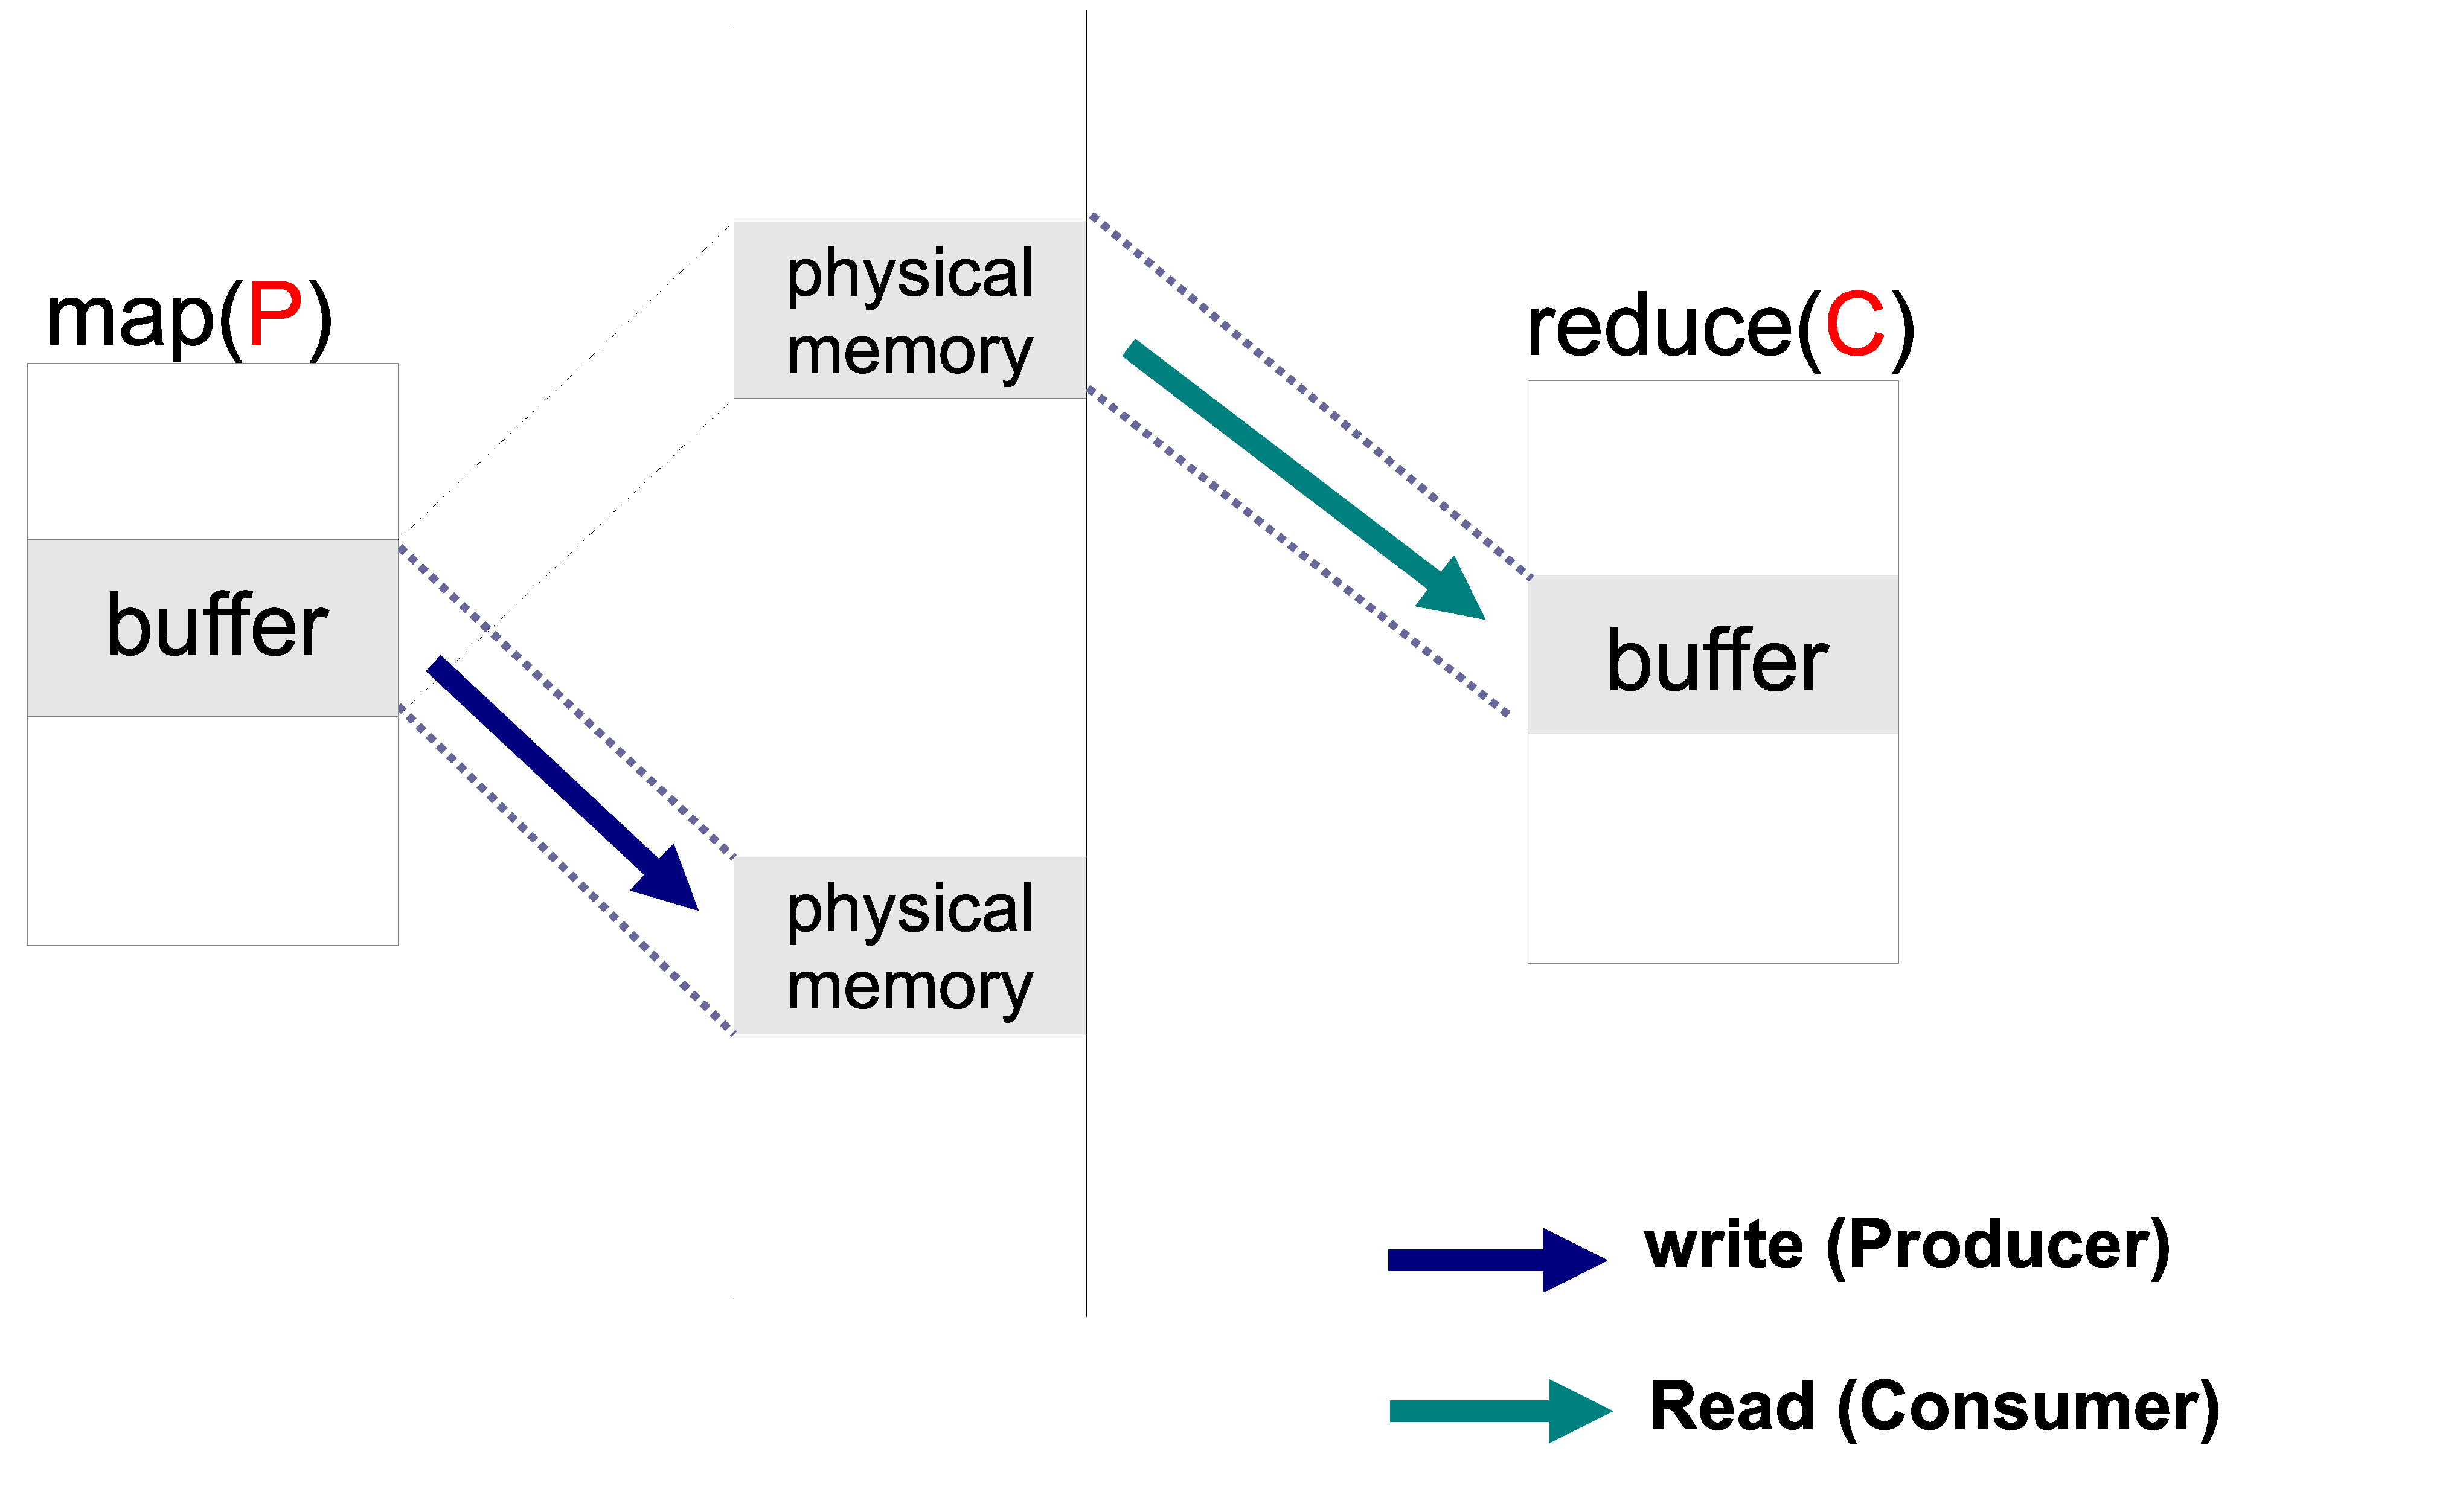
\includegraphics[width=0.5\textwidth]{img/dmr_pc_model.eps}
    \caption{producer-consumer model in DMR}
    \label{dmr:pc-model}
\end{figure}

如图\ref{dmr:pc-model}所示,综上所述,
DMR中producer-consumer模型的关键不同之处有两点:
其一,producer和consumer之间是一对一的隐式queue,
因此producer之间无须竞争,可以避免锁的竞争带来的开销。
其二,producer和consumer之间的隐式queue,
不采用显示的操作,而是采用一种mapping的方式,
即一旦buffer中的数据满,producer便会触发一个send操作,
底层的实现中,会将buffer对应的物理内存加入到隐式queue中,
buffer重新映射到一块新的物理内存,
producer只需将buffer设置为空,
便可继续对buffer进行读写。
这种方式的优点在于其快速高效。

DMR中的具体操作为,map worker向buffer中写入数据,
当buffer满时触发send操作,
之后将buffer标志为空,便可继续向buffer中写数据。
reduce worker以轮循的方式读取各个隐式queue中的数据,
从而,map worker和reduce worker可以并发的进行工作,
且不需要复杂的同步手段。
\input mapbuf
